\chapter{Background}
General discription of used terms/systems in wikipedia like style. This means the description should not be too extensive.
And refer to further papers for more extensive descriptions.
\section{Wireless Networks}
  \subsection{WLAN Channel}
    %https://de.wikipedia.org/wiki/Wireless_LAN#Frequenzen\newline
    \begin{description}
    \item[What is a Channel?]
    \item[Overview on useable frequencies]
    \item[Interference]
    \item[Hidden Station Problem]
    item[\ac{CSMA/CD}]
    \item[Analogy switch - collision domain]
    \end{description}
  \subsection{Wireless Access-Point}
    %Used to establish wireless connections to devices, like laptops/mobile phones, but also printer and ... 
    %Connecting wired LAN - wireless LAN \newline
    %Mostly provide access to internet\newline
    %Usecases of Accesspoints\newline
    %https://de.wikipedia.org/wiki/Wireless_Access_Point \newline
  \subsection{Wireless Mesh Network}
    %https://de.wikipedia.org/wiki/Ad-hoc-Netz
    %Topology for nodes(devices) in a wireless network.
    %Self healing capabilities.
    %Role of Mesh routers.
    %Redundancy in mesh networks.
    %Autonomy of devices.
    %Infrastructure mode vs p2p mode
    %IEEE 802.11
    %Alterations in our scenario compared to standard mesh\newline
    \cite{Akyildiz2005445}
    \cite{airberry}
    \subsection{Wireless Distribution System}
    %https://en.wikipedia.org/wiki/Wireless_distribution_system
    Description of WDS + AutoWDS \newline
      \begin{description}
       \item[What is a Wireless Distribution System?]
       How does the Lancom \ac{AutoWDS},differ from the basic WDS definition?
	 Intended centralized solution compüared to WDS systems due to better managability.
	 Also security is a key element for this system => that's why central entity + CAPWAP
      \end{description}
      \subsection{VLAN}
      \subsection{Spanning Tree + STP}
      \subsection{bandwidth}
      \subsection{BFS}
      \subsection{OpenVZ}
	\cite{openvz}
      \subsection{k-connectivity, k-edge-connectivity}
\section{Graph-theoretic Basics}
  Since we are using a graph based approahc in finding a solution we model a \ac{WMN} to a graph with a vertex set and an edge set. The goal is then to assign channels
  to the edges of this graph.
  %https://de.wikipedia.org/wiki/Graph_%28Graphentheorie%29
  TODO: Describe directed/undirected weighted graph
  What does connected graph mean; path
   \subsection{Mapping Data to Graph}
    For our solution we will use the following mapping from devices and modules to a undirected, weighted graph. (Formale beschreibung hilfreich?)
    Each accesspoint and each module of those accesspoints is represented by a node.
    For each accesspoint we add edges with the highest weight to each module of its corresponding accesspoint. 
    We describe those edges as artificial or device-module edges.
    If two modules of different accesspoints are within receive range of each other, 
    we are adding an edge between the corresponding module nodes with the average signal-to-noise ratio as the edge-weight.
    We call those edges module-module connections or real connections.
    Since the average of the two SNR's might not adequately represent the actual quality of those connections,
    we alternatively can easily adjust the edge-weight to the minimum or maximum of those values.
    While the average seems to be a good compromise for a general description of the underlying network, the minimum might be a better representation for 
    a more pessimistic setup, since the connection is then guaranteed to have at least this SNR in both directions. 
    Furthermore we are ignoring onesided connections, i.e. one module receives one or a few beacons of the other module but not the other way round.
    Not only are the SNRs of those connections mostly very poor, but they are also very rare in our target scenarios with omnidirectional antennas.
    So mostly either the modules receive each others beacons, or both do not.
    \begin{figure}[t]
      \centering
      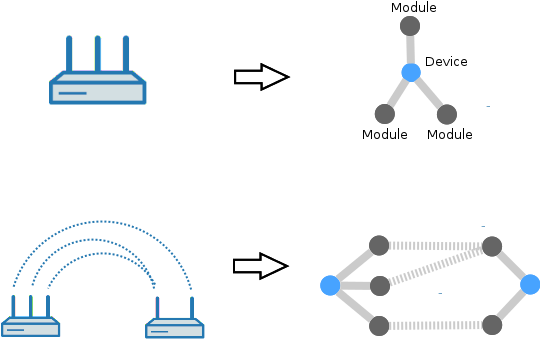
\includegraphics[width=0.5\columnwidth]{figures/apgraph.png}
      \caption{Graph representation of one and two connected accesspoints}
      \label{fig:apgraph}
    \end{figure}
   \subsection{Relevance of COLORING}
   \subsection{Dijkstra's Algorithm}
   TODO: How is our Channel assignment related to the problem COLORING?
    It is realated in the way that we want to assign each Module-Module-Connection a channel/color from a pool of available colors, withouth (if possible) use the same channel/color on neighboring links (meaning Aps that see each other and their traffic could lead to decreased throughput due to interference)
    Why is it not just coloring?
